\chapter{Statistics on the Sphere and Non-Gaussianities Detection}
\label{ch_fluctu}
\index{statistic}
\section{Introduction}
\index{CMB}
\index{detection!non-Gaussianity}
The search for non-Gaussian signatures in the cosmic microwave background (CMB) temperature fluctuation maps furnished by
MAP\footnote{http://map.gsfc.nasa.gov/} \citep{komatsu2003}, and to be furnished by PLANCK\footnote{http://astro.estec.esa.nl/SA-general/Projects/Planck/},
is of great interest for cosmologists. Indeed, the non-Gaussian signatures in the CMB can be related to very fundamental questions
such as the global topology of the universe \citep{riazuelo2002}, superstring theory, topological defects such as cosmic strings
\citep{gauss:bouchet88}, and multi-field inflation \citep{bernardeau2002}. The non-Gaussian signatures can, however, have a different 
but still cosmological origin. They can be associated with the Sunyaev-Zel'dovich (SZ) effect \citep{sunyaev80} (inverse Compton
effect) of the hot and ionized intra-cluster gas of galaxy clusters \citep{gauss:aghanim99,cooray2001}, with the gravitational 
lensing by large scale structures \citep{threepoint:bernardeau03}, or with the reionization of the universe \citep{gauss:aghanim99,castro2002}. 
They may also be simply due to foreground emission \citep{gauss:jewell01}, or to non-Gaussian instrumental noise and systematics \citep{banday2000}.
\index{SZ effect}
\index{cosmic strings}

All these sources of non-Gaussian signatures might have different origins and thus different statistical and morphological
characteristics. It is therefore not surprising that a large number of studies have recently been devoted to the subject 
of the detection of non-Gaussian signatures. Many approaches have been investigated: Minkowski functionals and the morphological 
statistics \citep{gauss:novikov00,gauss:shandarin02}, the bispectrum (3-point estimator in the Fourier domain) 
\citep{gauss:bromley99,gauss:verde00,gauss:phillips01}, the trispectrum (4-point estimator in the Fourier domain) \citep{gauss:kunz01}, 
wavelet transforms \citep{gauss:aghanim99,gauss:forni99,gauss:hobson99,gauss:barreiro01,gauss:cayon01,gauss:jewell01,starck:sta03_1}, 
and the curvelet transform \citep{starck:sta03_1}. In \citep{gauss:aghanim03,starck:sta03_1}, it was shown that the wavelet transform 
was a very powerful tool to detect the non-Gaussian signatures. Indeed, the excess kurtosis (4th moment) of the wavelet coefficients 
outperformed all the other methods (when the signal is characterized by a non-zero 4th moment). Based on kurtosis of wavelet coefficients, 
recent studies have reported non-Gaussian signatures in the WMAP data \citep{wave:vielva04,gauss:pia04,gauss:cruz05}.
The excess kurtosis is a widely used statistic, based on the 4th moment. 
% For any (symmetrical) random variable $X$, the kurtosis is:
% \[
% \kappa(X) = \frac{EX^4}{(EX^2)^2} -3. 
% \]
The kurtosis measures a kind of departure of $X$ from Gaussianity. The non-Gaussianty detector consists of first applying 
a multiscale transform (e.g., wavelet, or curvelet), and then calculating at each scale the kurtosis. In practice, missing 
data and instrumental effects may create an artificial kurtosis and it is very important to produce realistic simulations 
which present the same caracteristics as the observated data (e.g., missing data, noise, etc.). Then the kurtosis obtained 
from the data is compared to the kurtosis level expected from the simulations.
 
Finally, a major issue of the non-Gaussian studies in CMB remains our ability to disentangle all the sources of non-Gaussianity 
from one another. Recent progress has been made on the discrimination between different possible origins of non-Gaussianity. 
Namely, it was possible to separate the non-Gaussian signatures associated with topological defects (cosmic strings) from those 
due to the Doppler effect of moving clusters of galaxies (both dominated by a Gaussian CMB field) by combining the excess kurtosis 
derived from both the wavelet and the curvelet transforms \citep{starck:sta03_1}. 

The wavelet transform is suited to spherical-like sources of non-Gaussianity, and a curvelet transform is suited to structures 
representing sharp and elongated structures such as cosmic strings. Each provides an adapted non-Gaussian estimator, namely 
the normalised mean excess kurtosis. The combination of these transforms through the product of the normalized mean excess kurtosis 
of wavelet transforms by normalized mean excess kurtosis of curvelet transforms highlights the presence of the cosmic strings 
in a mixture CMB+SZ+CS. Such a combination gives information about the nature of the non-Gaussian signals. The sensitivity of 
each transform to a particular shape makes it a very strong discriminating tool \citep{starck:sta03_1,starck:jin05}.

\begin{figure}[htb]
\centering
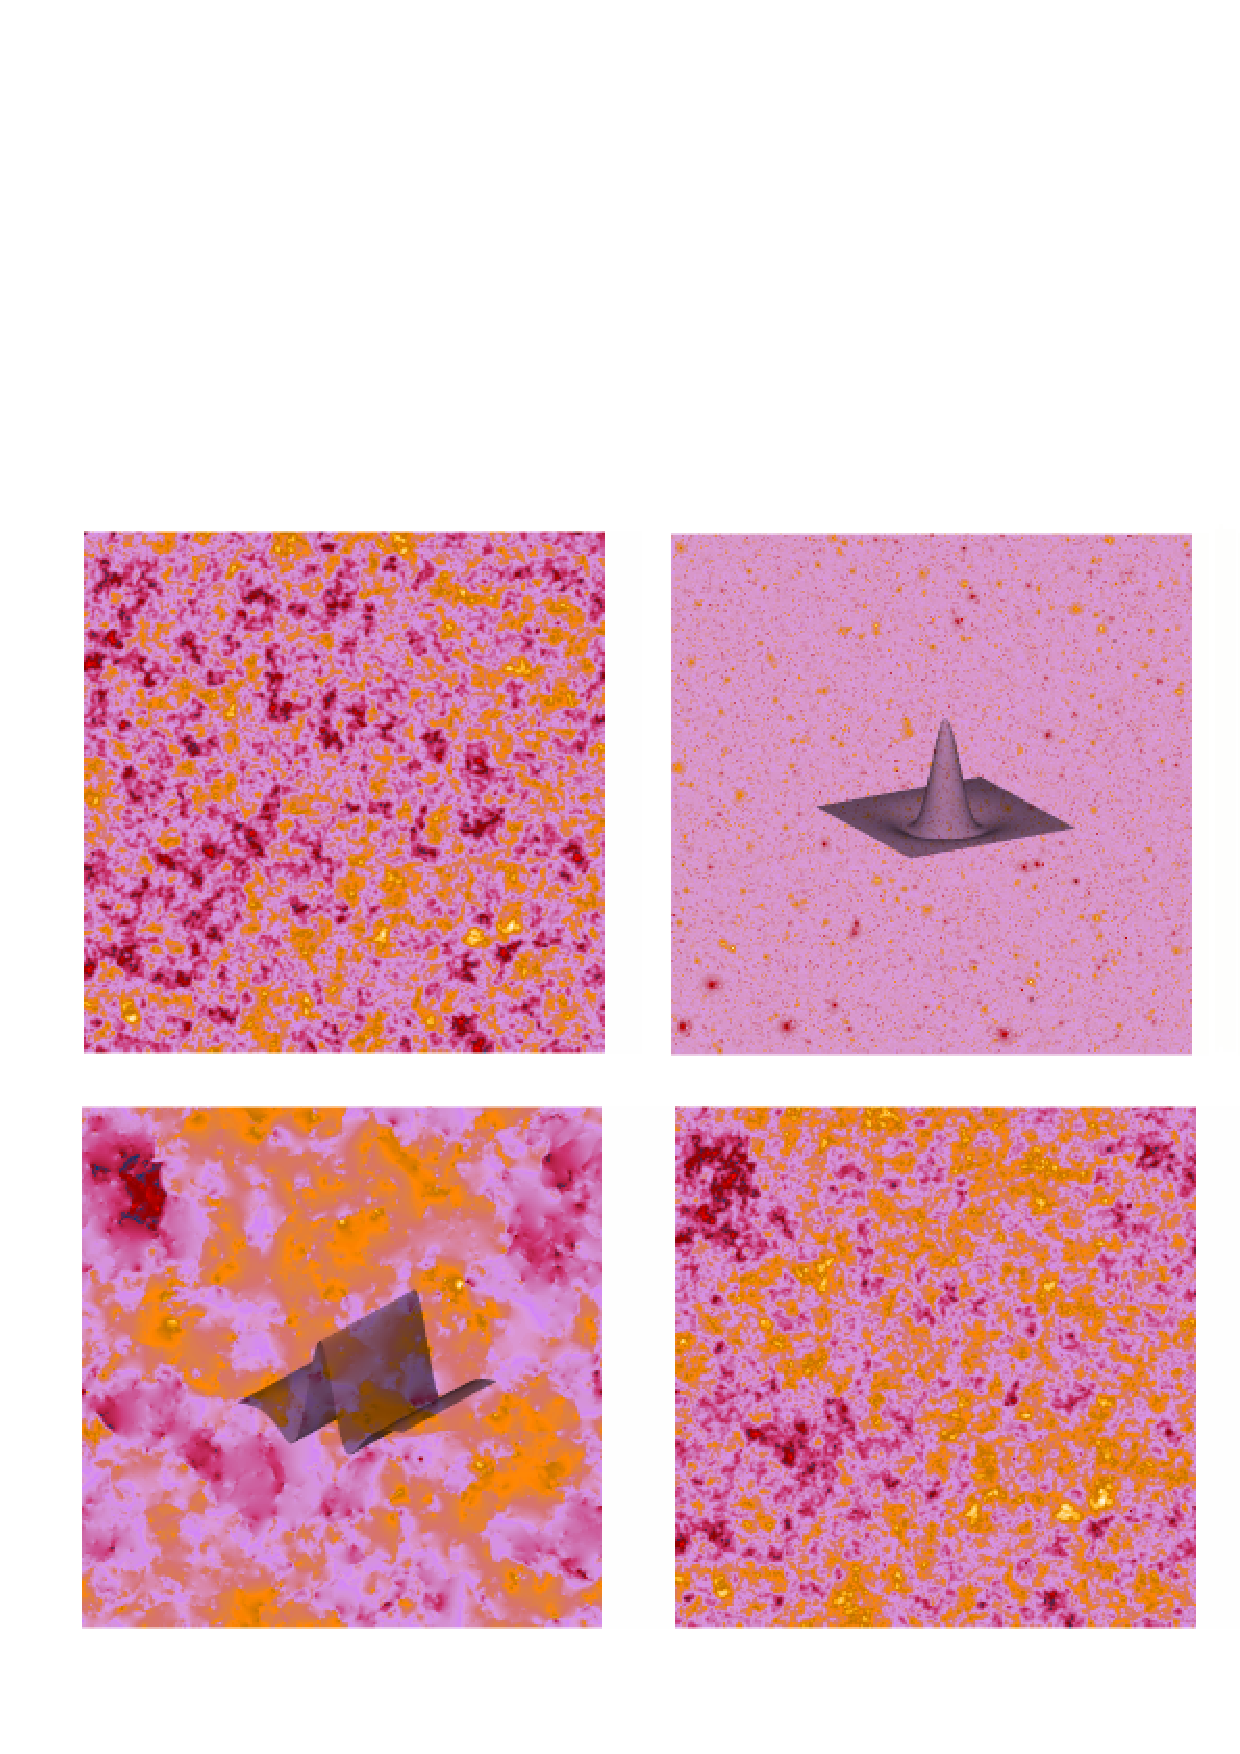
\includegraphics[width=13cm,height=13cm]{fig_cmbcssz.pdf}
\caption{Top, primary Cosmic Microwave Background anisotropies (left) and kinetic Sunyaev-Zel'dovich fluctuations (right). 
Bottom, cosmic string simulated map (left) and simulated observation containing the previous three components (right). 
The wavelet function is overplotted on the Sunyaev-Zel'dovich map and the curvelet function is overplotted on cosmic string map.}
\label{fig_cmb}
\end{figure}

In order to illustrate this, we show in Fig.~\ref{fig_cmb} a set of simulated maps. Primary CMB, kinetic SZ and cosmic string 
maps are shown respectively in Fig.~\ref{fig_cmb} top left, top right and bottom left. The ``simulated observed map", containing 
the three previous components, is displayed in Fig.~\ref{fig_cmb} bottom right. The primary CMB anisotropies dominate all the 
signals except at very high multipoles (very small angular scales). The wavelet function is overplotted on the kinetic Sunyaev-Zel'dovich 
map and the curvelet function is overplotted on cosmic string map.


CMB data are different from other astronomical data sets in the sense that they are not sparse (typical sparse data are stars or/and 
galaxies on top of a smooth background). After a component separation processing (see chapter~\ref{ch_mrs_ica}), the CMB data are not 
completely free of contaminations. Point sources still need to be detected and removed. Once we believe the data are clean enough, 
we want to check if the distribution of CMB temperature fluctuations is Gaussian by using robust statistical Gaussianity tests. 
\index{SZ effect}
\index{cosmic strings}
\index{CMB}

\section{Point Sources on a Gaussian Background}
\index{detection!point sources}
\index{wavelet!mexican hat}
\index{detection!matched filter}

Several methods have been proposed in the last years for point source detection in the CMB such as the the Mexican Hat wavelet \citep{gauss:cayon00,gauss:cayon01}, 
the pseudo-filter \citep{gauss:sanz01}, or the biparametric scale-adaptive filter \citep{gauss:sanz05}. A simple and robust technique, which maximizes 
the signal-to-noise ratio is the Matched Filter \citep{gauss:vio02}. Assuming an isotropic point spread function (PSF) with known power sprectum $\tau(q)$ 
and the CMB with power spectrum $P(q)$, the Matched Filter is \citep{gauss:vio02}:
\begin{equation} 
\label{eqn_mf}
\widehat{\psi}_{MF}(q) = \frac{1}{2 \pi \alpha}~ \frac{\tau(q)}{P(q)},\qquad \alpha \equiv \int_0^{+\infty}q \frac{\tau^2}{P} ~dq
\end{equation}
with minimum variance
\begin{equation} 
\sigma^2 = \frac{1}{2 \pi \alpha}
\end{equation}

\newpage
If the PSF is unknown (or space-variant), the Mexican Hat wavelet may be a good alternative. It consists of convolving the data 
with the wavelet function $\psi_{a,b} (x) =  \psi(\frac{x-b}{a})$, where $\psi(x)= \frac{1}{\sqrt{2\pi}}(1 - x^2) e^{- x^2/2}$. 
$a$ is the scale parameter and $b$ the position parameter. A fast implementation is obtained by using the Fourier transform to 
perform the convolution products ($\widehat{\psi}_{a}(q) = \frac{2}{\sqrt{\pi}} {(q a )}^2 e^{- \frac{1}{2}{(q a)}^2}$) \citep{gauss:sanz05}.




\section{Detecting Faint Non-Gaussian Signals Superposed on a Gaussian Signal}
\label{sec:Theory}
The superposition of a non-Gaussian signal with a Gaussian signal can be modeled as $Y = N + G$, where $Y$ is the observed image, 
$N$ is the non-Gaussian component and $G$ is the Gaussian component. We are interested in using transform coefficients to test 
whether $N \equiv 0$ or not.  

\subsection{Hypothesis Testing and Likelihood Ratio Test (LRT).}  
\label{subsec:LRT}
\index{statistic!LRT}

Transform coefficients of various kinds [Fourier, wavelet, curvelet, etc.] have been used for detecting non-Gaussian behavior 
in numerous studies. Let $X_1, X_2, \ldots, X_n$ be the transform coefficients of $Y$; we model these as  
\begin{equation}    
\label{EqAlt}
X_i = \sqrt{1 - \lam} \cdot  z_i + \sqrt{\lam} \cdot w_i,  \qquad 0< \lam < 1
\end{equation}
where $\lam >0$ is a parameter, $z_i \stackrel{iid}{\sim} N(0,1)$ are the transform coefficients of the Gaussian component $G$, 
$w_i \stackrel{iid}{\sim} W$ are the transform coefficients of the non-Gaussian component $N$, and $W$ is some unknown symmetrical 
distribution. Here without loss of generality, we assume the standard deviation for both $z_i$ and $w_i$ are $1$. 

Phrased in statistical terms, the problem of detecting the existence of a non-Gaussian component is equivalent to discriminating between the hypotheses:  
\begin{eqnarray}
\label{EqHypo2}
&H_0: \;\;\;   X_i = z_i  \label{EqHypo1}   \\
&H_1:   X_i = \sqrt{1 - \lam } \cdot z_i  + \sqrt{\lam} \cdot  w_i,   \qquad 0 < \lam < 1  
\end{eqnarray}
and $N \equiv 0$ is equivalent to $\lam \equiv 0$. We call $H_0$ the {\it null hypothesis $H_0$}, and $H_1$ the {\it alternative hypothesis}. 

% \begin{figure}
% \centering
% \includegraphics[height = 3 in]{PDF/CSDetectRegion.pdf}
% \caption{Detectable regions  in the $\alpha-r$ plane.  With $(\alpha,r)$ in the white region on the top or the undetectable region, all methods completely fail for detection. With $(\alpha,r)$ in the white region on the bottom,  both excess kurtosis and Max/HC are able to detect reliably.      While in the blue region to the left,  Max/HC is able to detect reliably, but excess kurtosis completely fails, and in the yellow region to the right, excess kurtosis is able to detect reliably, but Max/HC  completely fail.     }
% \label{Figure:Detect}
% \end{figure}

\begin{figure}[htb]
\centerline{
\hbox{
\includegraphics[width=12cm]{CSDetectRegion.pdf}%,height=12cm
% \psfig{figure=,bbllx=1.5cm,bblly=8.cm,bburx=19.5cm,bbury=23cm,height=6cm,width=7.5cm,clip=}
 }}
\caption{Detection Boundary in the $\alpha-r$ plane. The solid curve is the detection boundary of LRT, above which is not possible to detect, 
and below which it is possible to reliably detect, the dotted line segment and solid line segment together is the detection boundary for Kurtosis, 
the dotted curve and the solid curve together is the detection boundary of Max/HC. Right panel: detectable regions for Kurtosis, Max/HC.}
\label{Figure:Detect}
\end{figure}

When both $W$ and $\lam$ are known, then the optimal test for Problem (\ref{EqHypo1}) - (\ref{EqHypo2}) is simply 
the Neyman-Pearson Likelihood ratio test (LRT), \cite[Page 74 ]{Lehmann}. The size of $\lam = \lam_n$  for which 
reliable discrimination between $H_0$ and $H_1$ is possible can be derived using asymptotics. If we assume that 
the tail probability of $W$ decays algebraically, 
\begin{equation} \label{EqDefineAlg}
\lim_{x \goto \infty}   x^{\alpha}  P\{|W| > x\}  = C_{\alpha},  \qquad \mbox{$C_{\alpha}$ is a constant}
\end{equation}
(we say $W$ has a power-law tail), and we calibrate $\lam$ to decay with $n$, so that increasing amounts of data are offset by increasingly hard challenges: 
\begin{equation}   \label{EqDefineLam}
\lam = \lam_n  = n^{-r}  
\end{equation}
then there is a {\it threshold effect} for the detection problem (\ref{EqHypo1}) - (\ref{EqHypo2}). In fact, define:\\
\begin{equation} \label{EqDetectBoundary}
\rho^*_1(\alpha) = 
\left\{ \begin{array}{ll}
2/\alpha, &\   \  \alpha \leq 8 \\
1/4, &\     \       \alpha > 8
\end{array}
\right.
\end{equation}
then as $n \goto \infty$, LRT is able to reliably detect for large $n$ when $r < \rho^*_1(\alpha)$, and is unable to detect 
when $r > \rho^*_1(\alpha)$; this is proved in \citep{DJ04b}. Since LRT is optimal, it is not possible for any statistic to 
reliably detect when $r > \rho^*_1(\alpha)$. We call the curve $r = \rho^*_1(\alpha)$ in the $\alpha$-$r$ plane the 
{\it detection boundary}; see Figure \ref{Figure:Detect}.\\

In fact, when $r < 1/4$, asymptotically LRT is able to reliably detect whenever $W$ has a finite $8$-th moment, even without 
the assumption that $W$ has a power-law tail. Of course, the case that $W$ has an infinite $8$-th moment is more complicated, 
but if $W$ has a power-law tail, then LRT is also able to reliably detect if $r < 2/\alpha$. 

% One component of the above result is that, by assuming  $W$ has an 
% $\alpha$-algebraic tail 
% with $\alpha > 8$, then when $r < \frac{1}{4}$,  LRT is 
% able to reliably detect;  
% and when $r > \frac{1}{4}$, no statistic is able to detect.  
% It is interesting to notice here that, this part of the conclusion will still hold 
% when  
% the condition of requiring $W$ to have an algebraic tail is largely relaxed:  in 
% fact,  the same conclusion still holds if we only require $E[W^8] < \infty$.  It is 
% interesting to notice here that,  when $W$ has an $\alpha$-algebraic tail, 
% $E[W^8] < \infty$ if and only if $\alpha > 8$.

Despite its optimality, LRT is not a practical procedure. To apply LRT, one needs to specify the value of $\lam$ and 
the distribution of $W$, which seems unlikely to be available. We need non-parametric detectors, which can be implemented 
without any knowledge of $\lam$ or $W$, and depend on $X_i$'s only. In the next section, we are going to introduce three 
non-parametric detectors: excess kurtosis, Max and Higher Criticism (HC).   

\section{Kurtosis, HC from Wavelet and Curvelet Coefficients}
 
\subsection{Kurtosis}
\index{statistic!Kurtosis}
\index{Kurtosis}

For a statistic $T_n$, the $p$-value is the probability of seeing equally extreme results under the null hypothesis:
\[
p = P_{H_0} \{ T_n  \geq t_n(X_1,X_2, \ldots,X_n) \}
\] 
here $P_{H_0}$ refers to probability under $H_0$, and $t_n(X_1,X_2, \ldots,X_n)$ is the observed value of statistic $T_n$. 
Notice that the smaller the $p$-value, the stronger the evidence against the null hypothesis. A natural decision rule based 
on $p$-values rejects the null when $p < \alpha$ for some selected level $\alpha$, and a convenient choice is  $\alpha = 5\%$. 
When the null hypothesis is indeed true, the $p$-values for any statistic are distributed as uniform $U(0,1)$. This implies 
that the $p$-values provide a common scale for comparing different statistics. 

We now introduce two statistics for comparison. 

{\bf Excess Kurtosis ($\kappa_n$)}. Excess kurtosis is a widely used statistic, based on the $4$-th moment. 
For any (symmetrical) random variable $X$, the kurtosis is:
\[
\kappa(X) = \frac{EX^4}{(EX^2)^2} -3
\]
The kurtosis measures a kind of departure of $X$ from  Gaussianity, as $\kappa(z) =  0$.
Empirically, given $n$ realizations of $X$, the excess kurtosis statistic is defined as: 
\begin{equation}  \label{EqDefineK}
\kappa_n(X_1, X_2,\ldots,X_n)  = \sqrt{\frac{n}{24}} \biggl[ \frac{\frac{1}{n}\sum_i  X_i^4}{(\frac{1}{n}  \sum_i X_i^2)^2}  - 3  \biggr]
\end{equation} 
When the null is true, the excess kurtosis statistic is asymptotically normal:
\[
\kappa_n(X_1, X_2,\ldots,X_n)  \rightarrow_{w}  N(0,1), \qquad n \goto \infty
\]
thus for large $n$, the $p$-value of the excess kurtosis is approximately:
\[
\tilde{p} = \bar{\Phi}^{-1} (\kappa_n(X_1, X_2,\ldots,X_n))
\]
where $\bar{\Phi}(\cdot)$ is the survival function (upper tail probability) of $N(0,1)$. 

It is proved in \citep{DJ04b} that the excess kurtosis is asymptotically optimal for the hypothesis testing of \eqref{EqHypo1} - \eqref{EqHypo2} if 
\[
E [W^8] < \infty
\]
However, when $E[W^8] = \infty$, even though kurtosis is well-defined ($E[W^4] < \infty$), there are situations in which LRT 
is able to reliably detect but excess kurtosis completely fails. In fact, by assuming \eqref{EqDefineAlg} - \eqref{EqDefineLam} 
with an $\alpha < 8$, if $(\alpha,r)$ falls into the blue region of Figure~\ref{Figure:Detect}, then LRT is able to reliably detect, 
however, excess kurtosis completely fails. This shows that in such cases, excess kurtosis is not optimal; see \citep{DJ04b}. 

\subsection{Max}
\index{statistic!max}
\index{max}
The largest (absolute) observation is a classical and frequently-used non-parametric statistic:
\[
M_n =  \mmax(|X_1|,|X_2|,\ldots, |X_n|)
\] 
under the null hypothesis, 
\[
M_n  \approx \sqrt{2 \log n}
\]
and moreover, by normalizing $M_n$ with constants $c_n$ and $d_n$, the resulting statistic 
converges to the Gumbel distribution $E_v$, whose cdf is $e^{-e^{-x}}$:
\[
\frac{M_n - c_n}{d_n}  \rightarrow_{w}    E_v
\]
where approximately
\[
d_n = \frac{\sqrt{6} S_n}{\pi}, \qquad  c_n = \bar{X} - 0.5772 d_n 
\]
here $\bar{X}$ and $S_n$ are the sample mean and sample standard deviation of $\{X_i\}_{i=1}^n$ respectively. 
Thus a good approximation of the $p$-value for $M_n$ is:
\[
\tilde{p} =  \mathrm{exp}(-\mathrm{exp}(-\frac{M_n - c_n}{d_n}))
\]
We have tried the above experiment for $n = 244^2$, and found that taking $c_n = 4.2627$, $d_n = 0.2125$ gives a good approximation.  

Assuming \eqref{EqDefineAlg} - \eqref{EqDefineLam} and $\alpha < 8$, or $\lam = n^{-r}$ and that $W$ has a power-law tail 
with $\alpha < 8$, it is proved in \citep{DJ04b} that Max is optimal for hypothesis testing \eqref{EqHypo1} - \eqref{EqHypo2}. 
Recall if we further assume $\frac{1}{4} < r < \frac{2}{\alpha}$, then asymptotically, excess kurtosis completely fails; 
however, Max is able to reliably detect and is competitive to LRT. 

On the other hand, recall that excess kurtosis is optimal for the case $\alpha > 8$. In comparison, in this case, 
Max is not optimal. In fact, if we further assume $ \frac{2}{\alpha} < r < \frac{1}{4}$, then  excess kurtosis 
is able to reliably detect, but Max will completely fail. 

In Figure \ref{Figure:Detect}, we compared the detectable regions of the excess kurtosis and Max in the $\alpha$-$r$ plane. 

\subsection{Higher Criticism}
\label{sec:HC}
\index{statistic!Higher Criticism}
\index{Higher Criticism}

The Higher Criticism statistic (HC), was proposed in \citep{gauss:lin02}. To define HC first we convert the individual $X_i$'s 
into $p$-values for individual $z$-tests. Let $p_i = P\{ N(0,1) > X_i \}$ be the $i^{th}$ $p$-value, and let $p_{(i)}$ denote 
the $p$-values {\it sorted in increasing order}; the Higher Criticism statistic is defined as:
\[
       HC_{n}^* =  \max_{i}
         \biggl| \sqrt{n} [i/n  - p_{(i)}]/ \sqrt{p_{(i)} (1-p_{(i)})} \biggr|
\]
or in a modified form:
\[
HC_n^+  = \max_{\{i:  \; 1/n  \leq  p_{(i)} \leq  1 - 1/n \}}
         \biggl|   \sqrt{n} [i/n  - p_{(i)}]/ \sqrt{p_{(i)} (1-p_{(i)})}  \biggr|
\]
we let $HC_n$ refer either to $HC_n^*$ or $HC_n^+$ whenever there is no confusion. The above definition is slightly 
different from \citep{gauss:lin02}, but the ideas are essentially the same.

With an appropriate normalization sequence:
\[
a_n = \sqrt{2 \log \log n}, \qquad b_n = 2 \log \log n + 0.5 \log \log \log n - 0.5 \log (4 \pi)
\]
the distribution of $HC_n$ converges to  the Gumbel distribution $E_v^4$, whose cdf is $\mathrm{exp}(-4\mathrm{exp}(-x))$, \citep{Shorack}:
\[
a_n  HC_n - b_n  \rightarrow_w  E_v^4
\]
so the $p$-values of $HC_n$ are approximately:
\begin{equation}  
\label{EqHCP}
\mathrm{exp}(-4\mathrm{exp}( - [a_n HC_n - b_n]))
\end{equation}
For moderately large $n$, in general, the approximation in \eqref{EqHCP} is accurate for the $HC_n^+$, but not for $HC_n^*$.   

A brief remark comparing Max and HC. Max only takes into account the few largest observations, HC takes into account those outliers, 
but also moderate large observations. As a result, in general HC is better than Max, especially when we have unusually many moderately 
large observations. However, when the actual evidence lies in the middle of the distribution both HC and Max will be very weak.

% \section{The Genus and the Multiscale Genus}

\section{Experiments}

\begin{figure}[htb]
\vbox{
\centerline{
\hbox{
 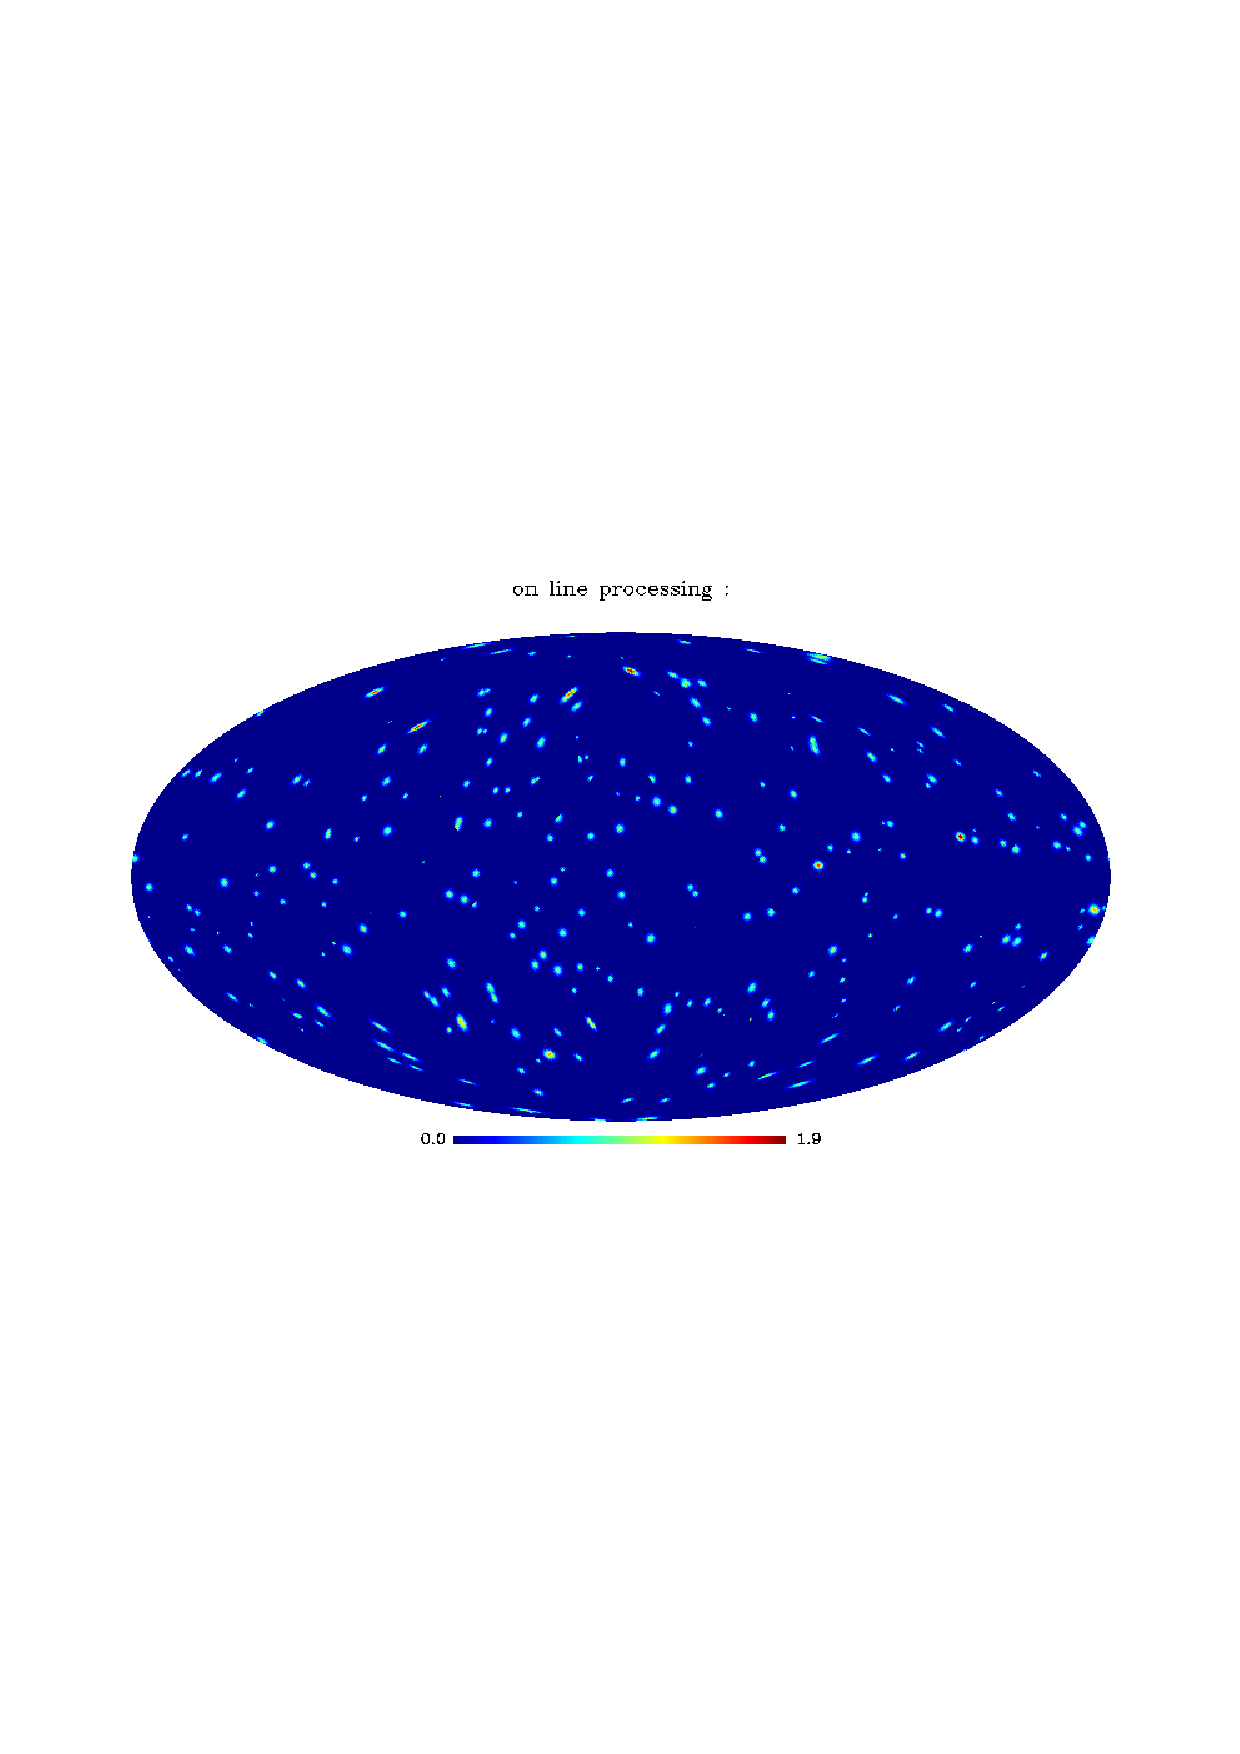
\includegraphics[trim= 2cm 8cm 2cm 8cm,width=7.9cm]{fig_sphere_gaussian.pdf}%[width=8.5cm,height=4.5cm]
 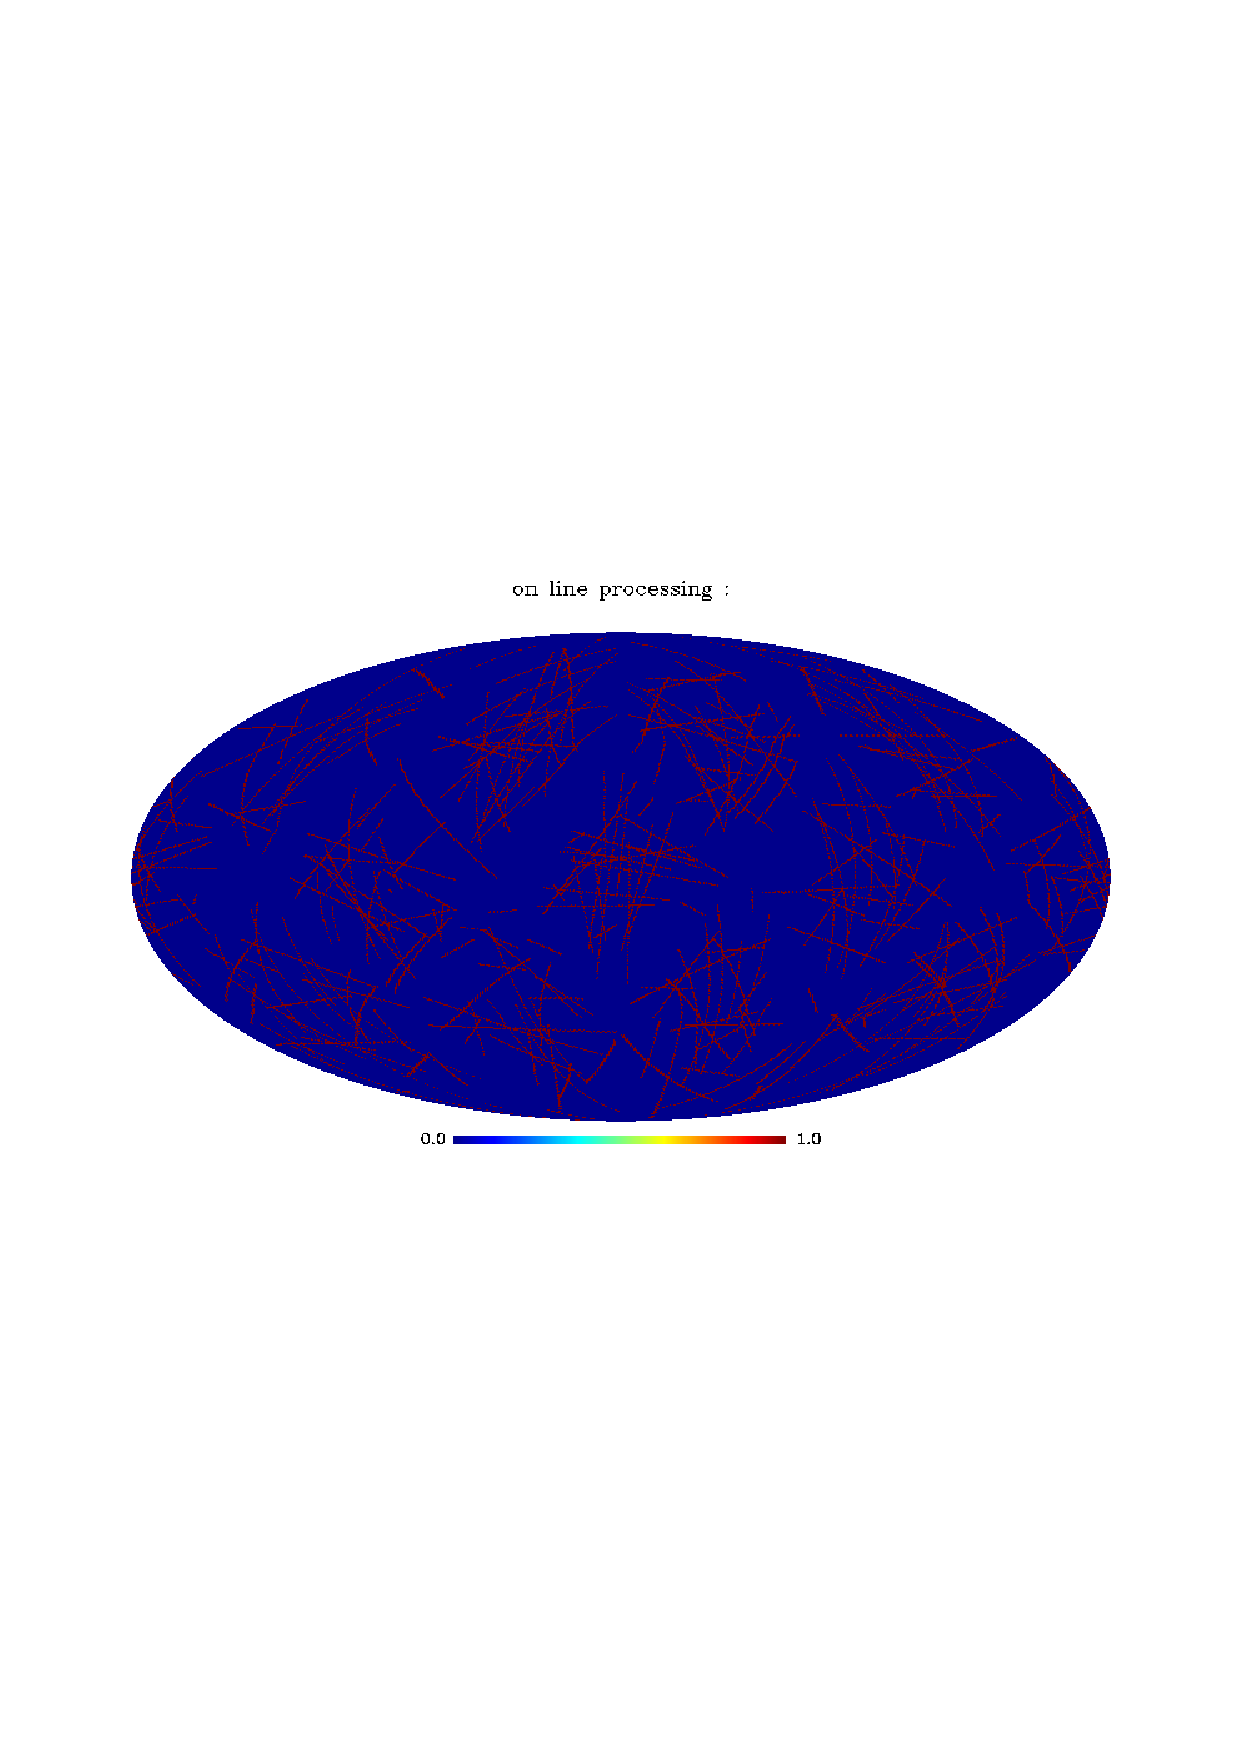
\includegraphics[trim= 2cm 8cm 2cm 8cm,width=7.9cm]{fig_sphere_line.pdf}
}}
 \centerline{
 \hbox{
 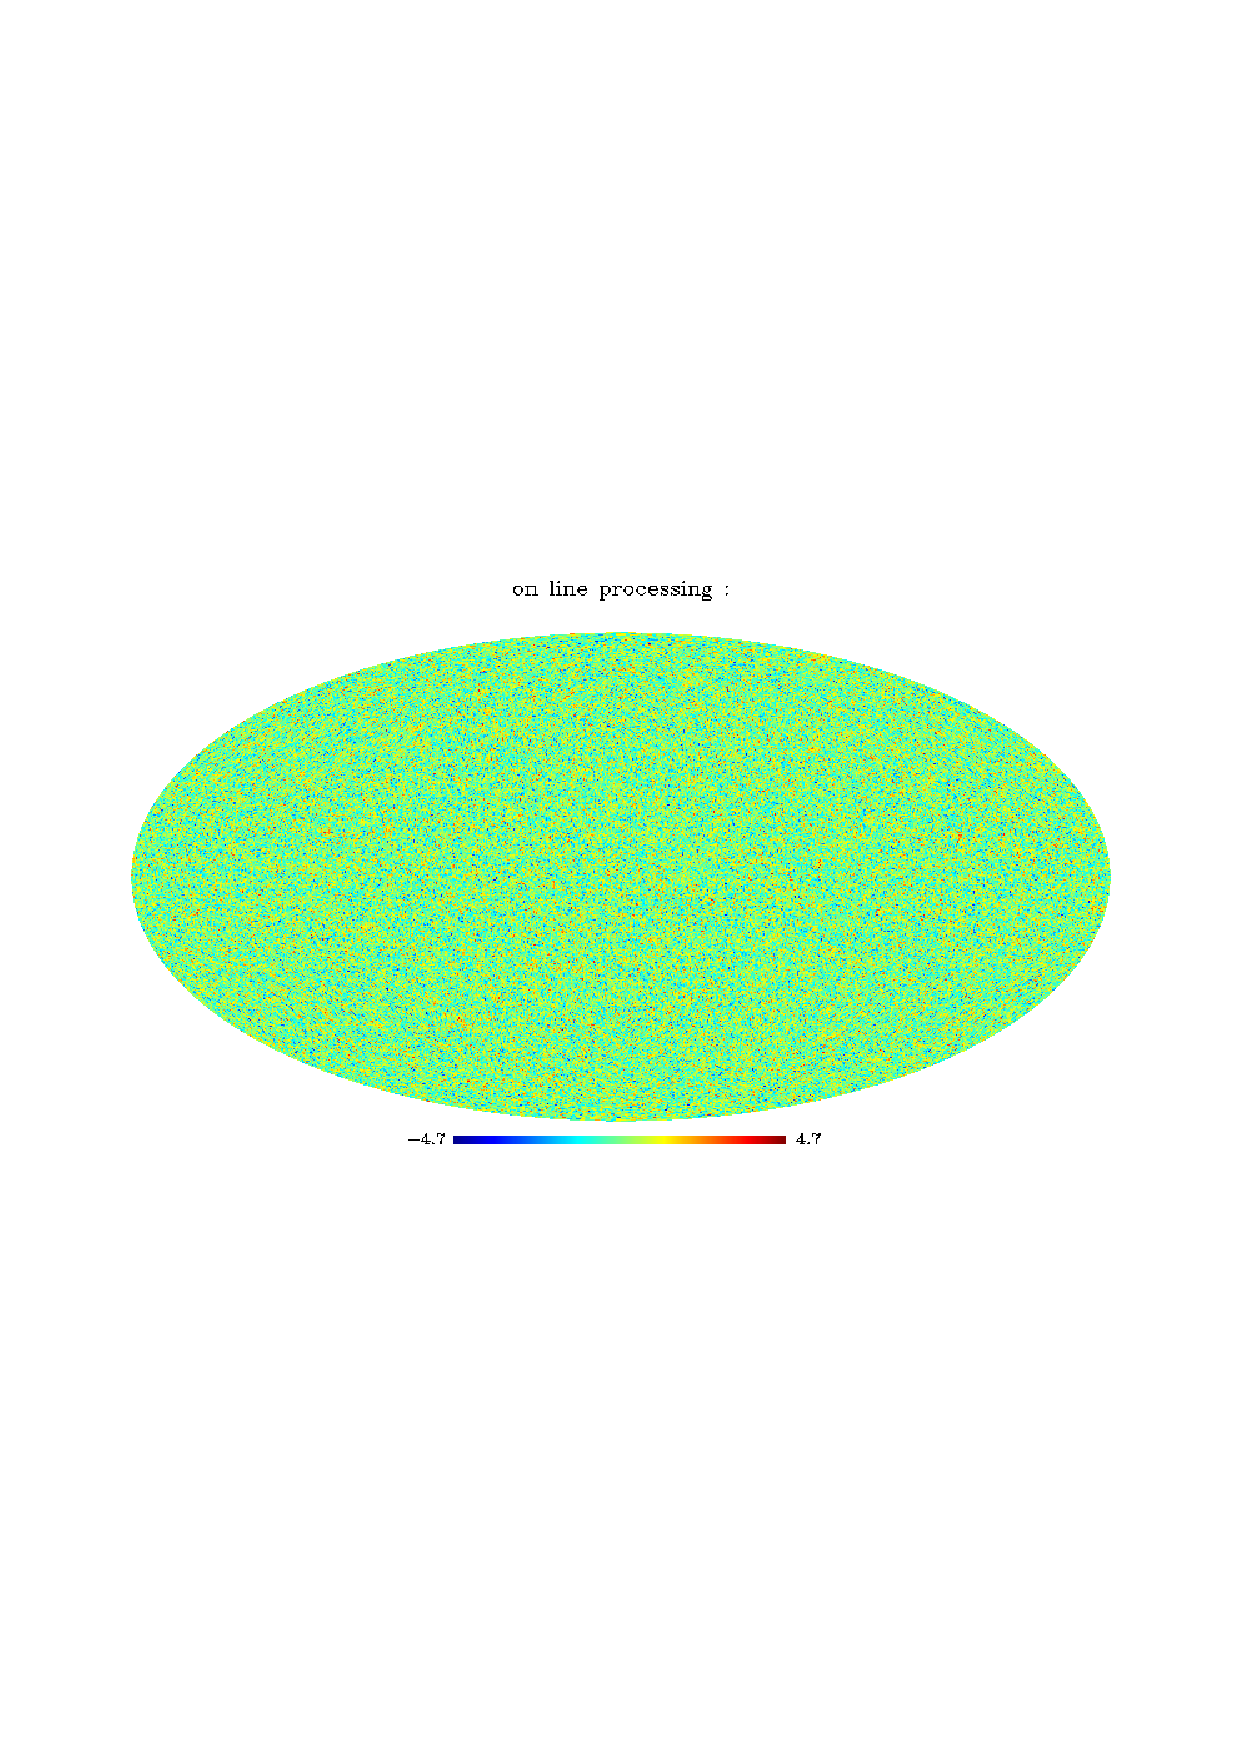
\includegraphics[trim= 2cm 8cm 2cm 8cm,width=7.9cm]{fig_sphere_gaussian_noise_snr1.pdf}
 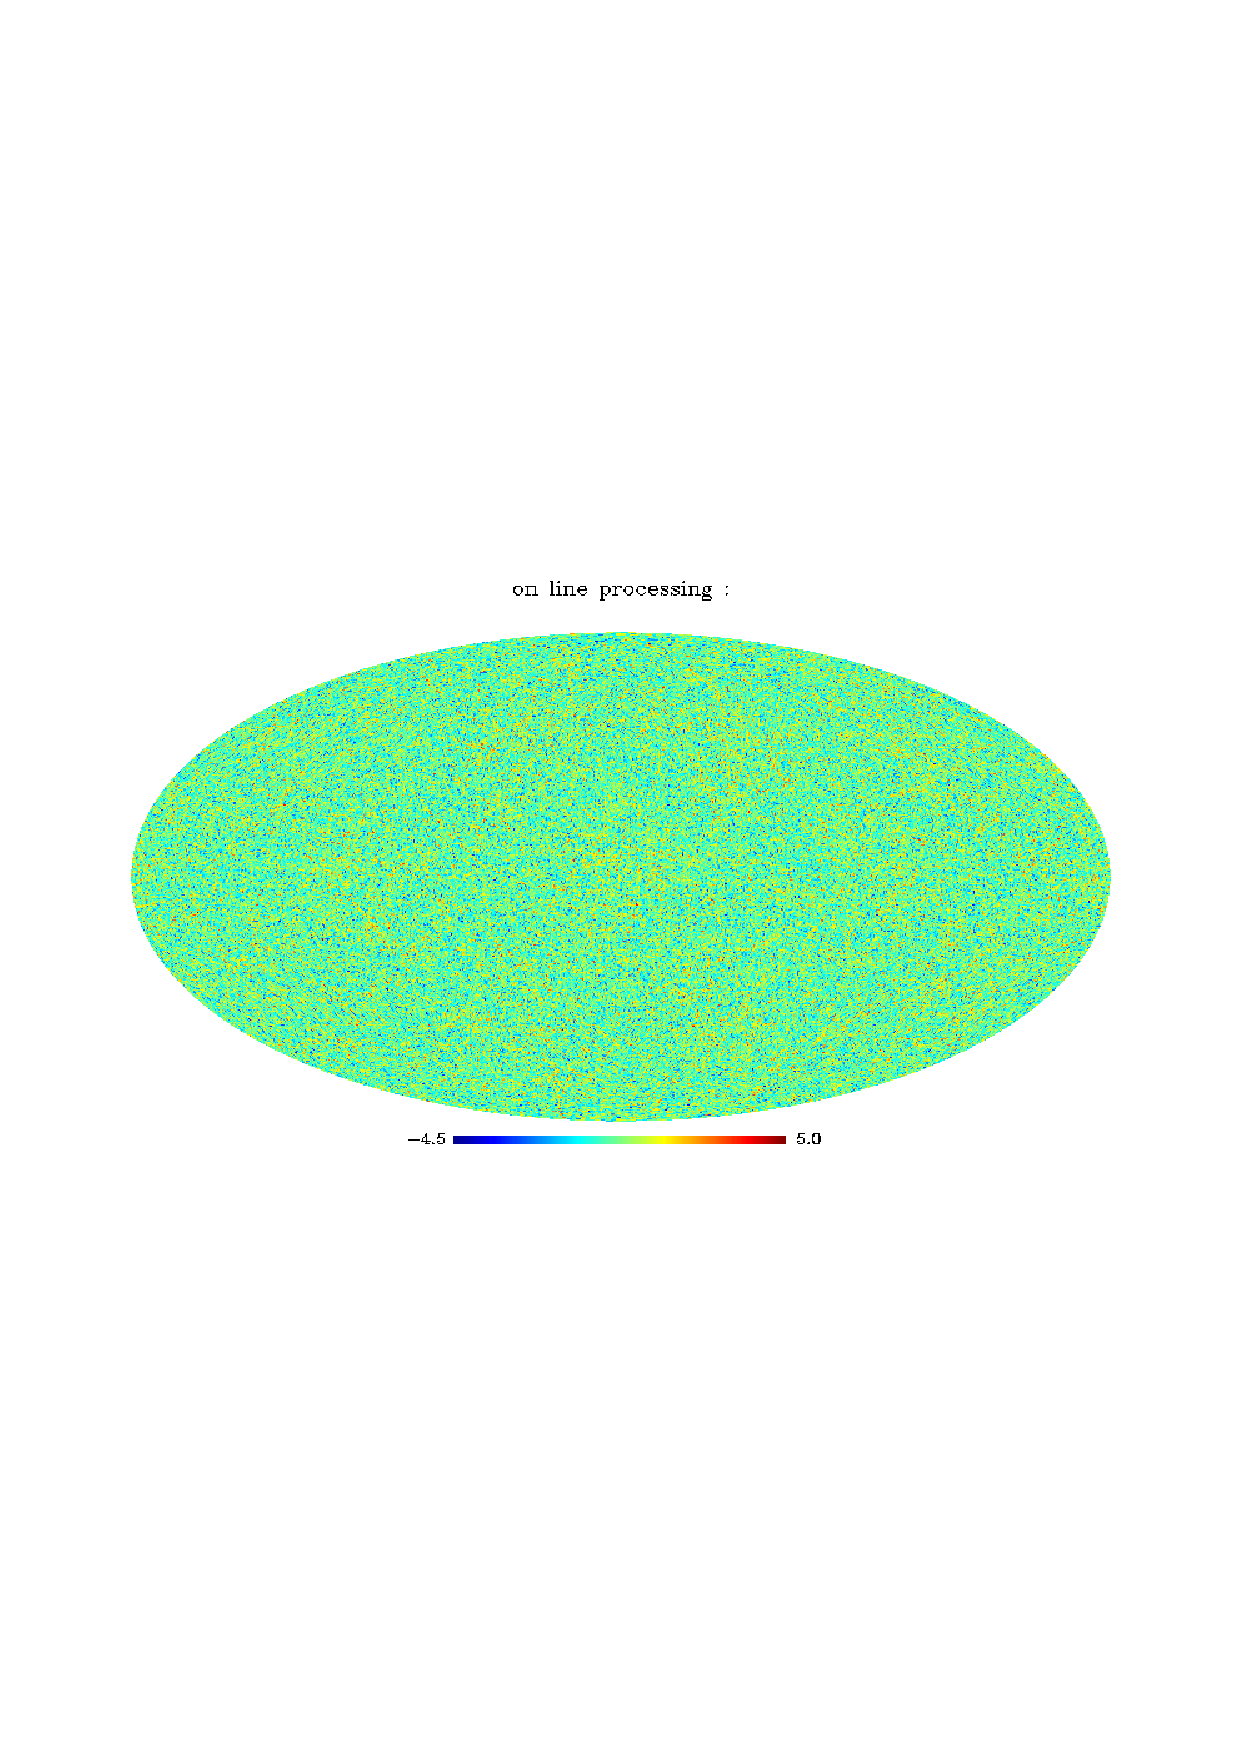
\includegraphics[trim= 2cm 8cm 2cm 8cm,width=7.9cm]{fig_sphere_line_noise_snr1.pdf}
}}}
 \caption{Top, image with Gaussians and image with lines. Bottom, same images but with an additional Gaussian noise. The SNR is equal to 1.}
\label{fig_sphere_linegauss}
\end{figure}

Fig.~\ref{fig_sphere_linegauss} shows, top left and right, two images with respectively Gaussians and lines. We have created a set 
of simulated images by adding a Gaussian white noise with different standard deviations to these two images. The Signal to Noise 
Ratio (SNR) varies between 0 and 1. For the image with lines, the SNR is defined as the pixel values along the lines divided by the 
noise standard deviation, and  for the image with Gaussians, the SNR is defined as the maximum of the Gaussians divided by the noise 
standard deviation. Fig.~\ref{fig_sphere_linegauss} shows, bottom left and right, the two noisy images with a SNR equal to 1. Hence, 
for each SNR value, we have thirty realizations of the noise, and we have calculated the kurtosis at the different scales of both the 
curvelet and the wavelet coefficients. These kurtosis values were normalized by the standard deviation of the kurtosis obtained from 
the wavelet and the curvelet transform of thirty Gaussian white noise realizations. Finally we kept for each SNR the maximum normalized 
kurtosis along the scales. Fig.~\ref{fig_wtcur_sphere_linegauss} left (resp.~right) shows the normalized kurtosis values using the wavelet 
transform (resp. the curvelet transform) for the two images (i.e. lines and Gaussians) versus the SNR. Continuous error bars correspond 
to $1\sigma$ level and dashed error bars correspond to $2\sigma$ level. We can clearly see that the detection power of the wavevet 
transform is much larger than the detection power of the curvelet transform for detecting non-Gaussianities due to isotropic features, 
while curvelets are more powerful than wavelets for detecting anisotropic features.

\begin{figure}[htb]
\centerline{
 \hbox{
% {figure=,bbllx=2.5cm,bblly=12.5cm,bburx=19.5cm,bbury=25.5cm,width=8.5cm,height=6.5cm,clip=}
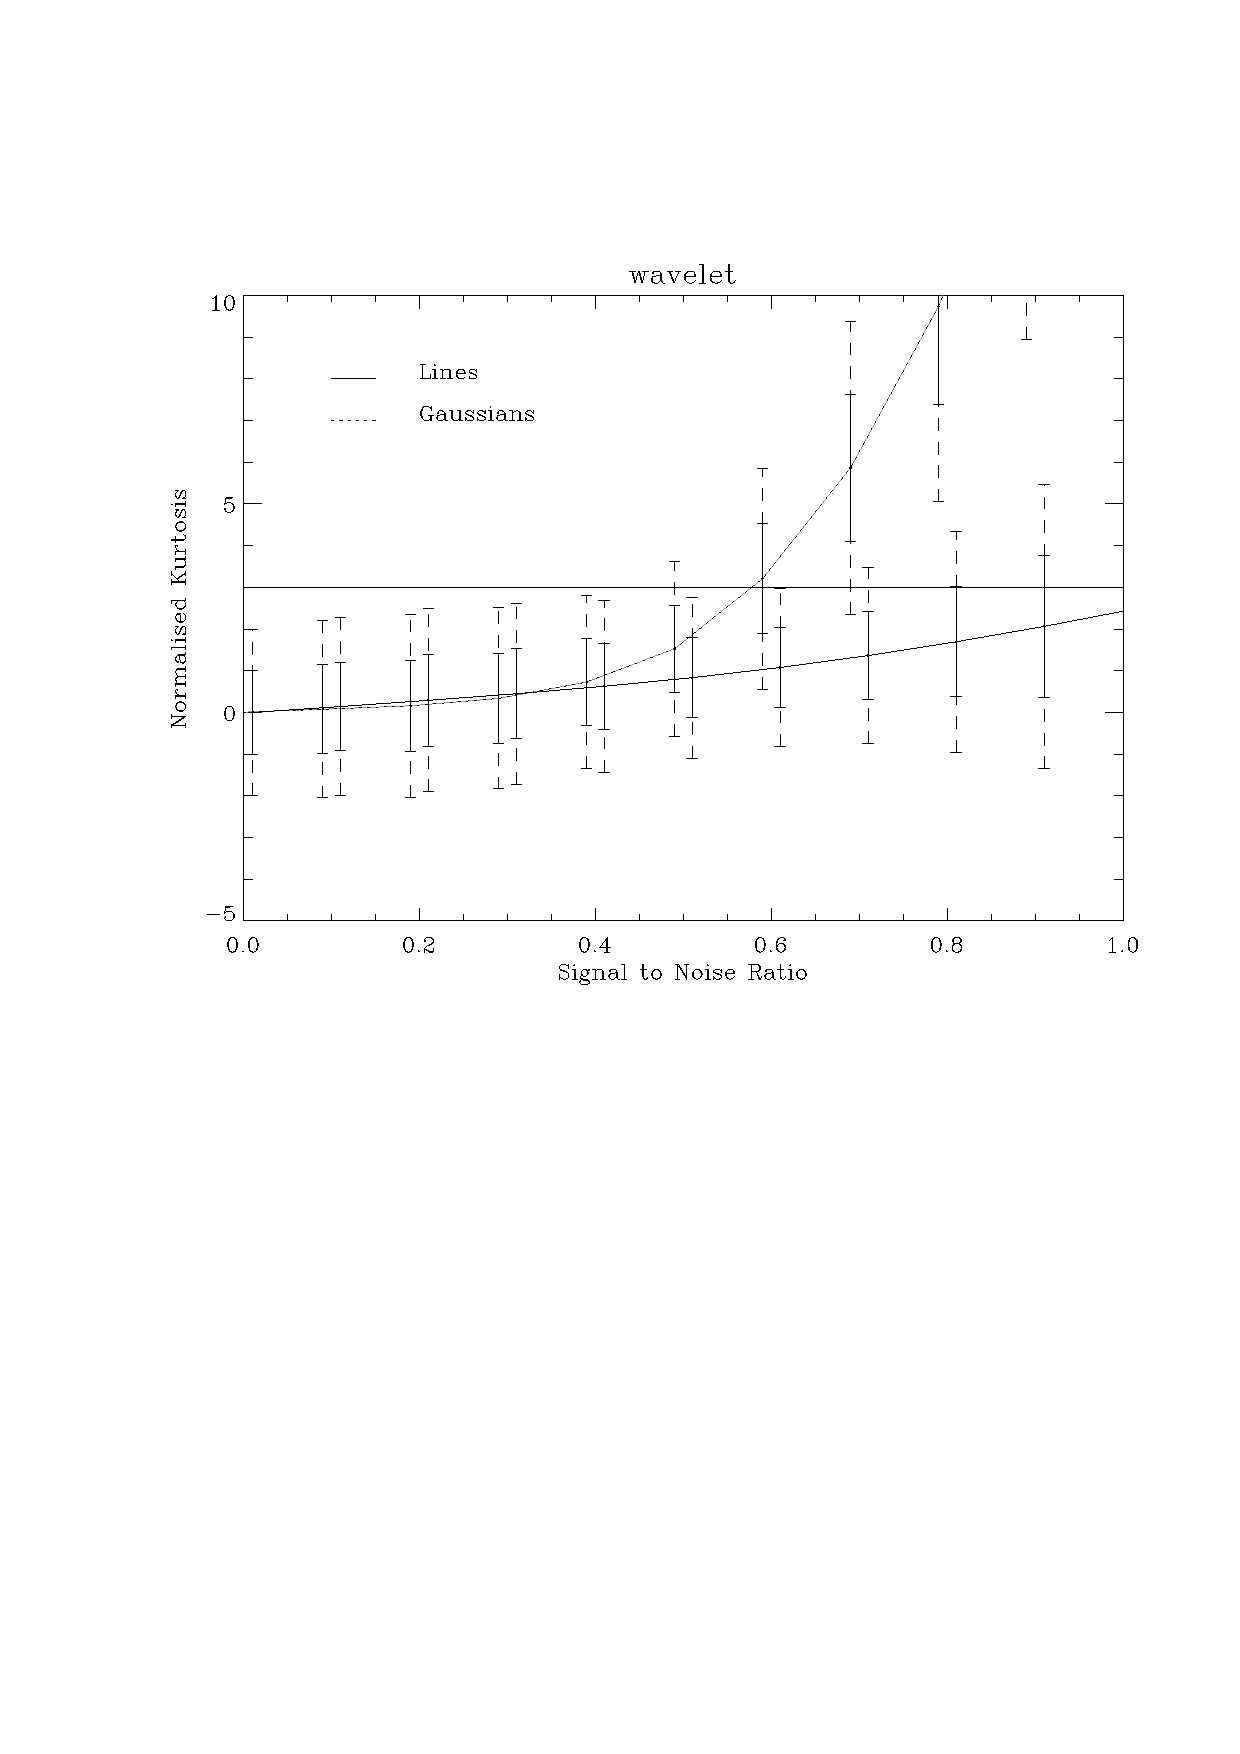
\includegraphics[trim= 2cm 13cm 2cm 3cm,width=7.9cm]{fig_sphere_wt_linedroite.pdf}%,height=6.5cm
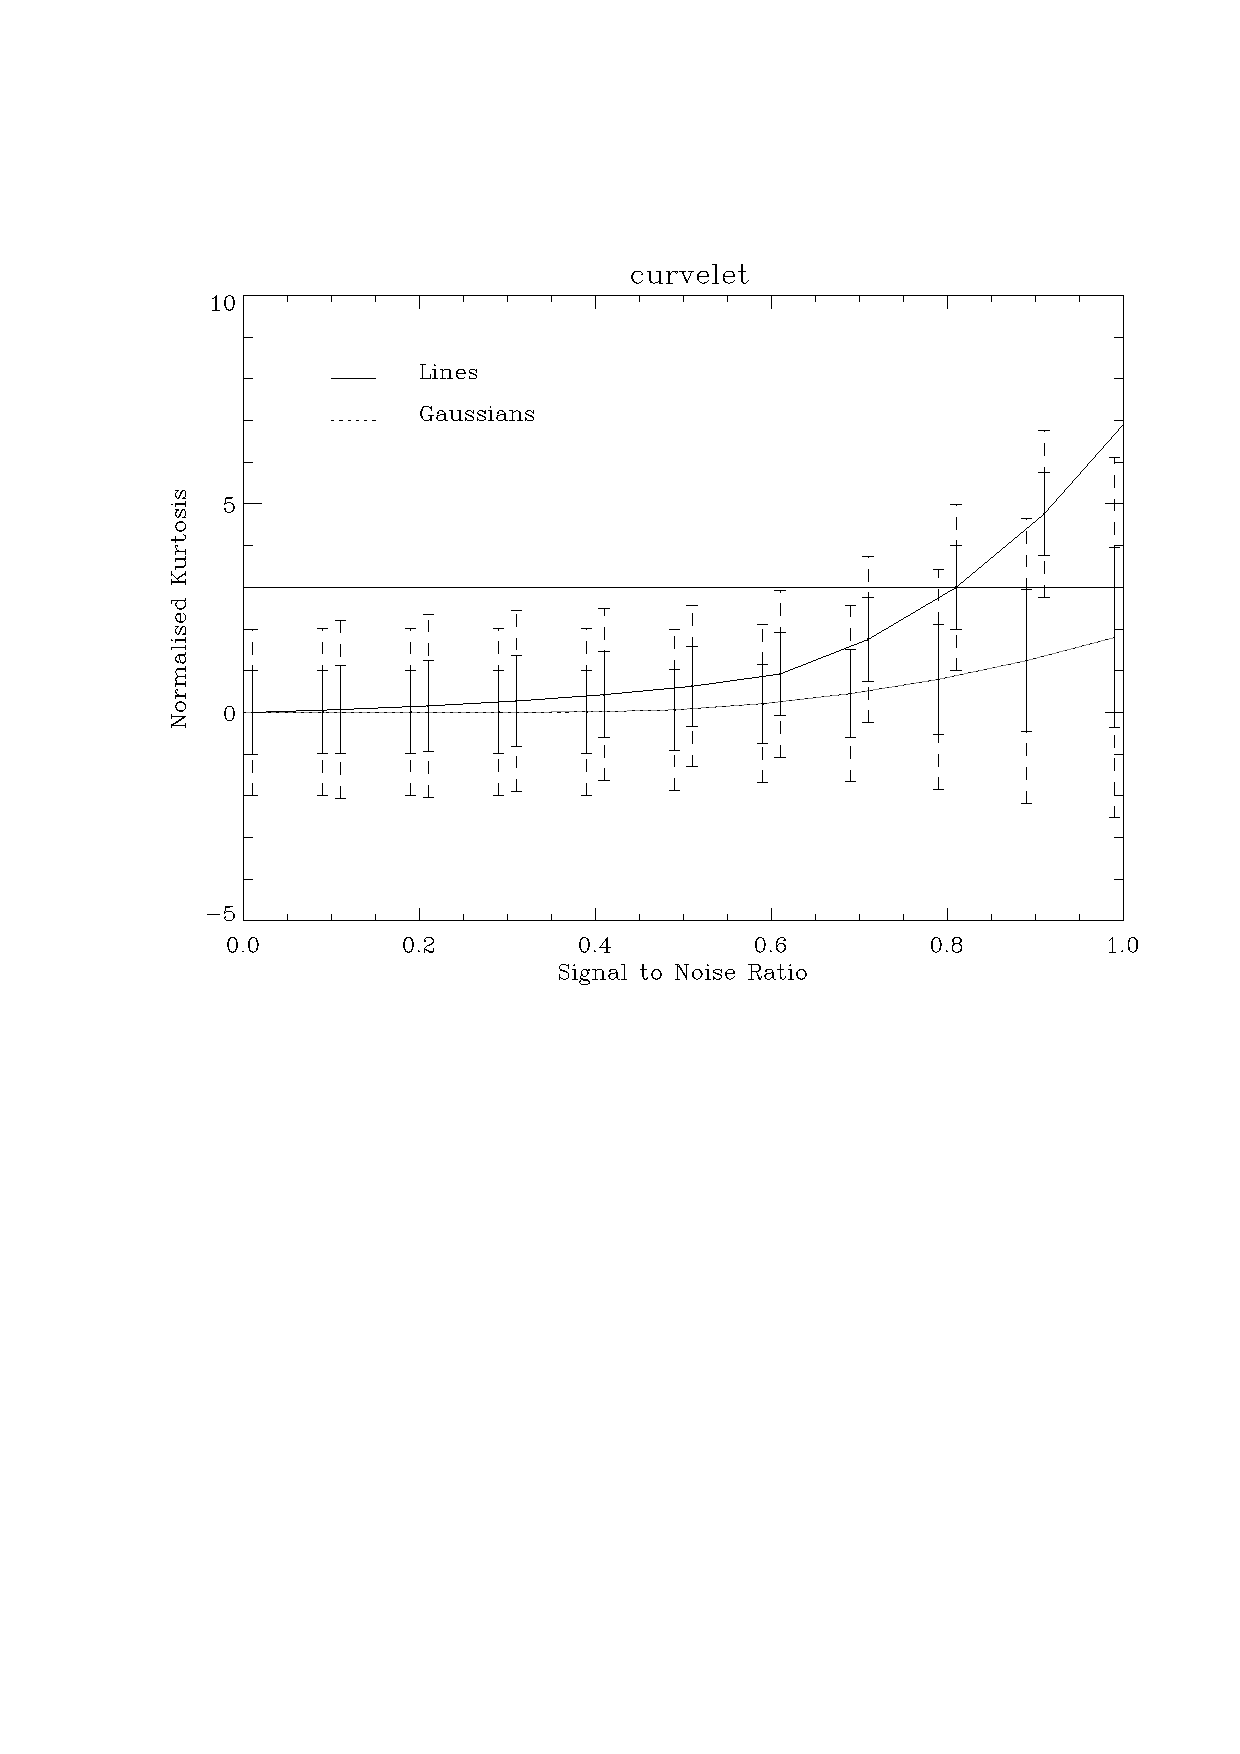
\includegraphics[trim= 2cm 13cm 2cm 3cm,width=7.9cm]{fig_sphere_cur_linedroite.pdf}
% \psfig{figure=fig_sphere_cur_linedroite.pdf,bbllx=2.5cm,bblly=12.5cm,bburx=19.5cm,bbury=25.5cm,width=8.5cm,height=6.5cm,clip=}
}}
\caption{Normalised kurtosis value versus the SNR for the wavelet coefficients (left) and the curvelet coefficients (right). 
The continuous error bars correspond to one $\sigma$ and the dashed error bars correspond to $2\sigma$.}
\label{fig_wtcur_sphere_linegauss}
\end{figure}

\section{Conclusions}
\index{wavelet!Kurtosis}
\index{wavelet!Higher Criticism}
\index{curvelet!Kurtosis}
\index{curvelet!Higher Criticism}
\index{SZ effect}
\index{cosmic strings}
\index{detection!non-Gaussianity}

The kurtosis of the wavelet coefficients is very often used in astronomy for the detection of non-Gaussianities in the CMB. It has been 
shown \citep{starck:sta03_1} that it is also possible to separate the non-Gaussian signatures associated with cosmic strings from those 
due to SZ effect by combining the excess kurtosis derived from these both the curvelet and the wavelet transform. It has been shown that 
kurtosis is asymptotically optimal in the class of weakly dependent symmetric non-Gaussian contamination with finite 8-th moments, while 
HC and MAX are asymptotically optimal in the class of weakly dependent symmetric non-Gaussian contamination with infinite 8-th moment \citep{starck:jin05}. 
Hence depending on the nature of the non-Gaussianity, a statitic is better than another one. This is a motivation for using several statistics 
rather than a single one for analysing CMB data. The case of the detection of cosmic string contaminations has been studied on simulated maps, 
and it has been shown that kurtosis outperforms clearly Max/HC \citep{starck:jin05}.  




